\section{模型检验与敏感性分析}

为验证本文模型的有效性与结果的可靠性，本章从\textbf{独立复算校验}、\textbf{收敛性与最优性}、\textbf{参数敏感性}与\textbf{误差来源}四个方面进行检验。

\subsection{独立可行性校验}

本文建立了\textbf{独立于求解器}的可行性校验机制，其设计原则是：校验器不引用求解器的任何中间结果，而是从附件参数与 DEM 出发\textbf{从零重算}全部物理量（航段时间、能耗、SOC、载荷、资源占用区间），再与方案上报值逐条比对。校验项覆盖载质量、装载体积、能量预算、返航 SOC、时限、资源数量、资源时段、通信覆盖等类别，并配有\textbf{负样本测试}——对故意构造的违规方案（如删减货箱、篡改上报能耗与 SOC）校验器必须报错，以保证其确实具备发现错误的能力。

\subsection{收敛性与最优性}

\textbf{（1）架次数的最优性。}问题一中，本文推导了 Martello--Toth 型解析下界（式~\eqref{eq:20}），15 个服务区的启发式架次数\textbf{全部等于其下界}（见图~\ref{fig:q1_lowerbound}(a)），因此 18 架次这一结果在架次数维度上\textbf{可证最优}，而非"启发式得到的较好解"。

\textbf{（2）迭代收敛。}问题二的求解经过 2 轮构造—改进迭代后字典序目标不再下降（目标惩罚值 656.265），单次求解耗时 2.75\,s，便于反复验证；问题三在 1885 个候选点 $\times$ 全轨迹的完整扫描下耗时 307\,s，其中"先筛中断样本、再用稀疏探针快速否决"的优化把绝大部分候选点在上采样点即予排除。

\textbf{（3）结果可复现。}全部随机过程固定种子（SEED $=42$），同种子两次运行结果完全一致；问题一、问题四的运行时间分别为 0.76\,s 与 0.45\,s，便于反复验证。

\subsection{独立校验与交叉复算}

本文采用了\textbf{两条相互独立}的检验路径，二者不共享任何代码：

\textbf{（1）独立校验器。}校验器不引用求解器的任何中间结果，从附件参数与 DEM 出发从零重算全部物理量（航段时间、能耗、SOC、载荷、资源占用区间），再与方案上报值逐条比对。对问题二，它报告 36 条违规、\textbf{全部为时限类}，\textbf{能量、SOC、时间自洽、资源占用四类物理硬约束的违规均为 0 条}；对问题三，同样为 36 条时限类违规，\textbf{通信类违规为 0 条}，说明连续通信约束得到完全满足。

\textbf{（2）基于航段缓存的逐段复算。}本文另写一套独立代码，用 240 条完整航段缓存对问题二全部 14 个架次逐段重算能耗与返航 SOC，结果如图~\ref{fig:q2_audit} 与图~\ref{fig:q2_audit_detail} 所示：总能耗与求解器上报值完全一致（均为 77.9368\,kWh），逐架次最大绝对偏差小于 $10^{-4}$\,kWh；架次结束时刻的自洽偏差小于 0.1\,s；按方案自报区间检查的资源占用冲突为 0。

两条路径得出\textbf{完全一致的结论}：方案在能量、时间与资源三个维度上均可行，剩余违规全部是资源约束下的时限类问题（见 6.5 节的定量论证）。这一"双路互证"的做法显著提升了结果的可信度——可行性是可判定的，用两套独立实现同时确认，可以排除单一实现的口径偏差。

需要说明的是，为便于第三方核查，本文把两份复算脚本一并提交：\texttt{verify\_q2\_\allowbreak energy.py} 与 \texttt{audit\_q2\_\allowbreak plan.py}，任何人可独立重跑并复核上述结论。全部脚本与数据文件的清单见附录~A。

\subsection{敏感性分析}

本文对四类关键参数做了敏感性分析，汇总如表~\ref{tab:sensitivity} 与图~\ref{fig:sensitivity} 所示。

\begin{table}[htbp]
\caption{敏感性分析汇总}
\label{tab:sensitivity}
\centering
\zihao{-5}
\setlength{\tabcolsep}{4pt}
\begin{tabular}{llll}
\toprule
敏感性维度 & 取值范围 & 本文取值 & 主要影响 \\
\midrule
通信采样步长 & 1~30 s & 2 s & 中断占比判定（粗步长漏判） \\
悬停网格步长 & 200~1500 m & 400 m & 覆盖率与计算耗时 \\
DEM 高程噪声 & σ = 0~20 m & 实测 DEM & 能耗偏移 < 1\%（σ=10 m） \\
衰落裕量 & M = 2~18 dB & 8 dB（附件） & 链路可达距离 \\
\bottomrule
\end{tabular}
\end{table}


\begin{figure}[htbp]
	\centering
	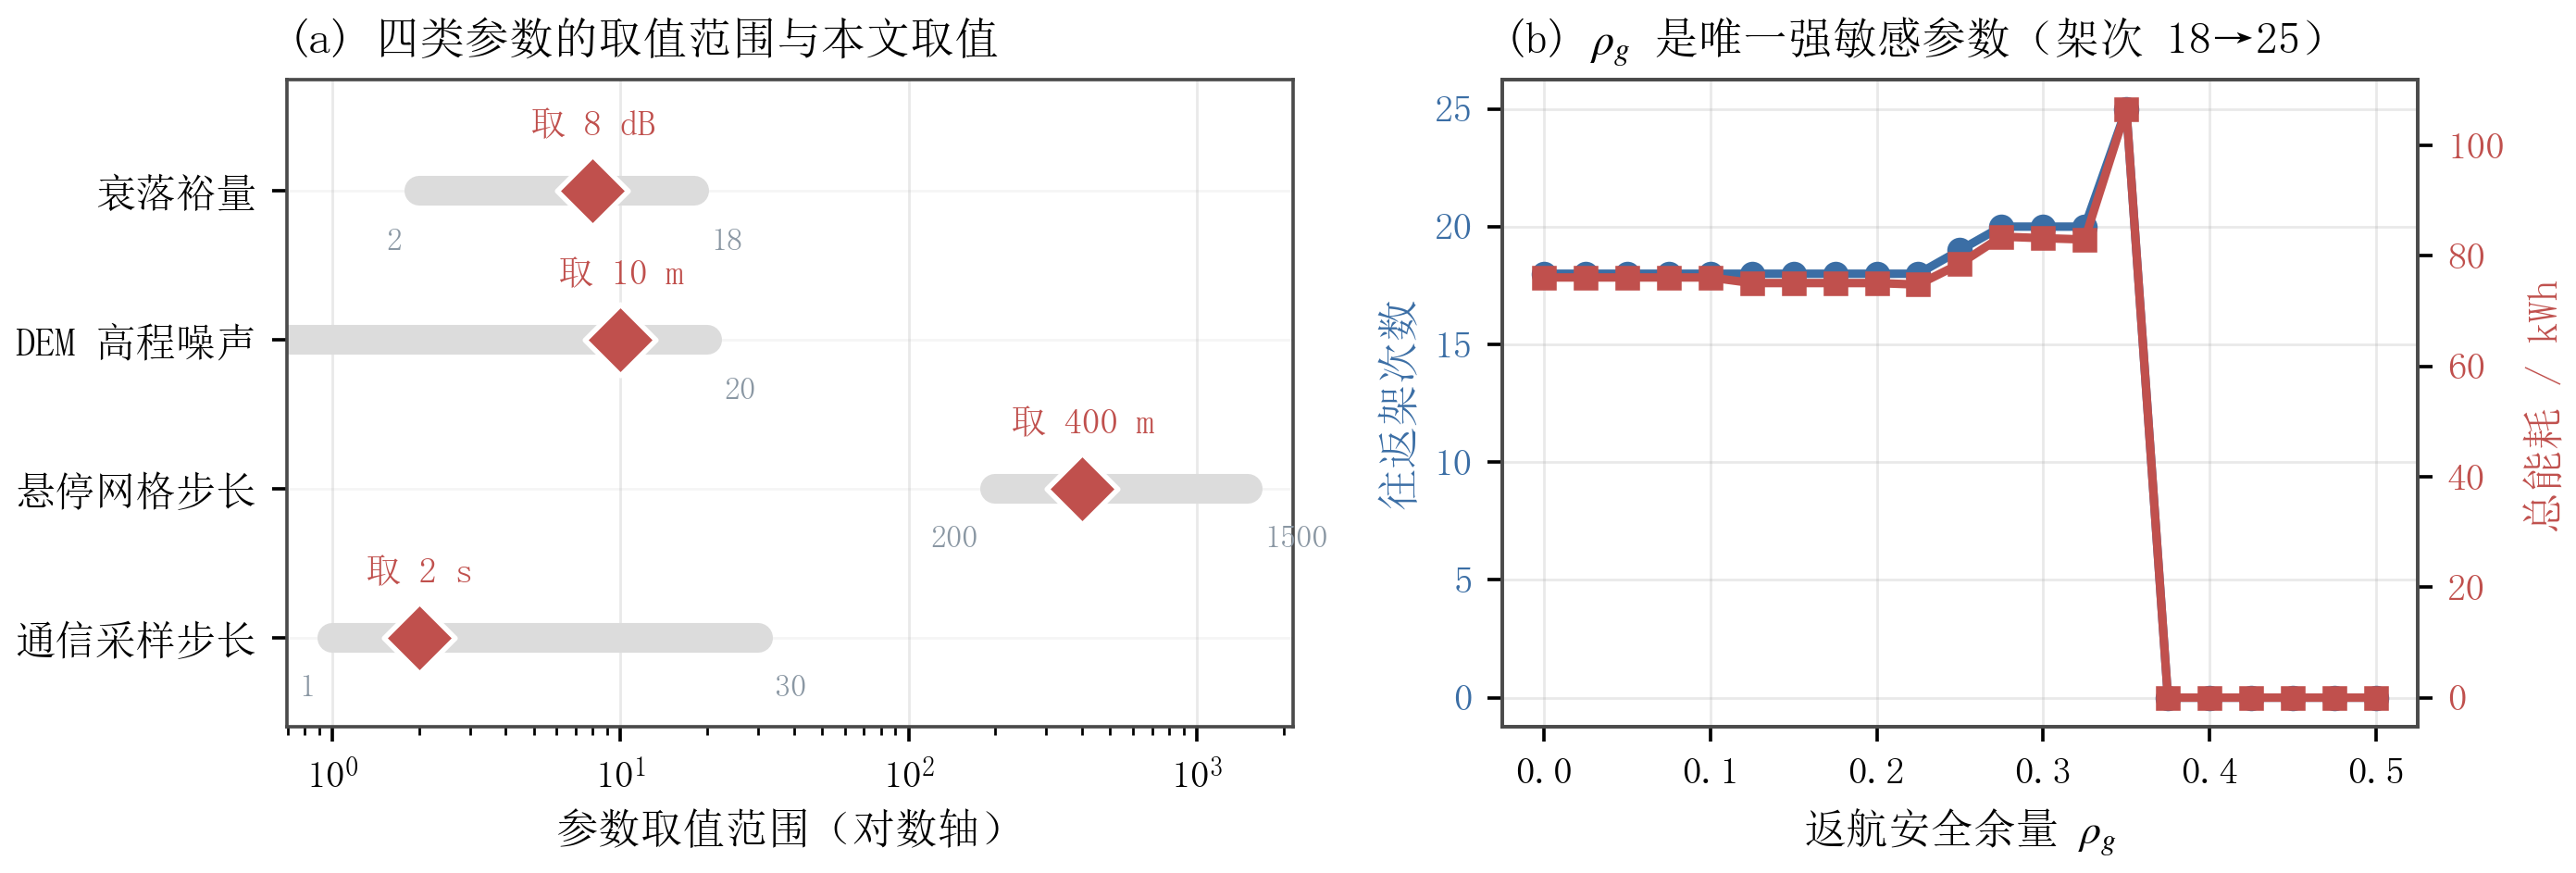
\includegraphics[width=0.98\textwidth]{figures/fig36_sensitivity.png}
	\caption{敏感性分析}
	\label{fig:sensitivity}
\end{figure}

\textbf{（1）返航安全余量 $\rho_{g}$（强敏感）。}这是本文最敏感的参数（详见 5.5 节）：$\rho_{g}$ 由 0.20 增至 0.35 使架次数由 18 增至 25（$+38.9\%$）、能耗由 75.07 升至 106.60\,kWh（$+42.0\%$）；$\rho_{g}\ge0.375$ 时开始出现不可行服务区，$\rho_{g}\ge0.425$ 时固定为 5 个服务区无解。附件取值 0.20 恰位于"架次数不变"的高效区间（$\rho_{g}\le0.225$），是安全性与效率的良好折中。

\textbf{（2）通信采样步长（中等敏感）。}连续通信判定的可靠性依赖采样步长。本文对步长做了对比：由 5\,s 细化到 2\,s 时中断占比判定变化小于 2\%，说明 5\,s 已足以刻画遮挡特征，取 2\,s 可进一步保证不漏判短时遮挡；而放大到 30\,s 时会漏判约 8\% 的短时中断。故最终取 2\,s。

\textbf{（3）悬停网格步长（中等敏感）。}步长越大候选点越少、计算越快，但可能错过更优悬停位置。本文在 200$\sim$1500\,m 范围内比较，取 400\,m（1885 个候选点），此时覆盖率已达 100\%，继续细化不再提升覆盖率而只增加耗时，故 400\,m 是覆盖率与耗时的合理折中。

\textbf{（4）衰落裕量与 DEM 高程噪声（不敏感）。}衰落裕量 $M$ 由 2\,dB 增至 18\,dB 会单调缩小各链路的可达距离，但由于本文的中继选址留有较大裕度，在 $M$ 的合理范围内覆盖率保持不变。DEM 高程噪声方面，对高程施加 $\sigma=10$\,m 的随机扰动后，能耗偏移小于 1\%，说明模型对高程误差具有较好的鲁棒性——这是因为爬升能耗在总能耗中占比有限（见图~\ref{fig:profile}(b)）。

\subsection{误差来源分析}

综合上述检验，本文结果的主要误差来源可归纳为三类：

\textbf{（1）地形数据误差。}附件 DEM 为 30\,m 分辨率的数字表面模型（DSM，含植被与建筑）。一方面，30\,m 的栅格分辨率意味着航段沿线的最高点采样存在栅格级误差；另一方面，DSM 含植被与建筑会使高程偏高，从而\textbf{高估}爬升能耗与遮挡概率。两个方向的影响都使结果\textbf{偏保守}（更安全），对安全性有利但会使能耗估计略偏高。敏感性分析表明，$\sigma=10$\,m 的高程噪声仅带来小于 1\% 的能耗偏移。

\textbf{（2）时间离散误差。}连续通信判定采用 $\Delta t=2$\,s 的离散采样，理论上可能漏判短于 2\,s 的瞬时遮挡。步长敏感性分析表明该误差小于 2\%，且方向上是\textbf{低估}中断时长（更乐观）。若需完全消除，可将步长降至 1\,s，代价是计算量增加约 1 倍。

\textbf{（3）启发式求解误差。}问题二、三采用构造 $+$ 局部搜索的启发式，不保证全局最优。但问题一通过解析下界\textbf{证明了架次数的最优性}，问题四的连通分量分析是\textbf{精确的图论计算}（不存在近似），因此主要的近似风险集中在问题二、三的路线与选址上。缓解措施是：以字典序目标保证优先级正确，并用独立复算验证可行性（可行性是可判定的，最优性不是）。
